\documentclass{article}

\usepackage{a4wide}
\usepackage[utf8]{inputenc}
\usepackage[T1]{fontenc}
\usepackage[french]{babel}
\usepackage[babel=true]{csquotes} % guillemets français
\usepackage{graphicx}
\graphicspath{{Images/}}
\usepackage{color}
\usepackage{hyperref}
\hypersetup{colorlinks,linkcolor=,urlcolor=blue}

\usepackage{amsmath}
\usepackage{amssymb}
\usepackage{fancyhdr}
\usepackage{xcolor}
\colorlet{RED}{red}
\pagestyle{fancy}

\renewcommand{\headrulewidth}{1pt}
\fancyhead[L]{\LaTeX \quad}
\fancyhead[C]{\textbf{page \thepage}} 
\fancyhead[L]{\leftmark}
\fancyhead[R]{Dodo'Cuisto}

\renewcommand{\footrulewidth}{1pt}
\fancyhead[L]{\LaTeX \quad}
\fancyfoot[C]{\textbf{page \thepage}} 
\fancyfoot[L]{L3 Info}
\fancyfoot[R]{\leftmark}

\title{APPLICATION MOBILE}
\author{DOYEN ROMAIN, DUCHEMAN MARQUES, L3 informatique}
\date{\today}

\begin{document}
\maketitle \center \textcolor{red}{Dodo'Cuisto}

\begin{center}
    
\includegraphics[scale=0.6]{logo.png} 
\end{center}

\newpage

%% Le résumé:
\begin{abstract}

\title{\textcolor{red}{Vue globale et but de l’application}}\\

En tenant compte des différentes exigences requises et notées dans le document de CCTP, nous avons décidé de développer une application de cuisine dont le but principal serait de consulter des recettes de cuisines créoles que d’autres utilisateurs ont postés.\\

C’est un sujet qui nous a beaucoup inspirés car étant passionné de cuisine, nous voulions faire partager la cuisine réunionnaise à un grand nombre de personne. L’île de la Réunion étant une île quasiment isolée dans l’Océan Indien, nous voulions faire exporter les spécialités locales à travers le monde.\\ 

L’application permettra à un utilisateur de :
\begin{itemize}
    \item \textbf{rechercher une recette :} Faire une recherche de recette disponible dans l’application
    \item \textbf{créer un compte :} Il faut obligatoirement s’inscrire pour pouvoir consulter, ajouter, modifier ou supprimer des recettes. Il peut également se déconnecter de son compte \textbf{Dodo’Cuisto}.
    \item \textbf{sauvegarder en favoris :} Permet de sauvegarder en favoris les recettes préféré de l’utilisateur.
    \item \textbf{consulter les recettes :} Permet de consulter les recettes affichées sur la page d’acceuil
    \item \textbf{modifier les recettes :} Permet d’ajouter, modifier ou supprimer les recettes
\end{itemize}

\end{abstract}

\newpage

%==============================================================================%

\tableofcontents

%\section{Introduction}
%\subsection{Technologies et outils utilisés}

%\section{Présentation de l’application}
%\subsection{Fonctionnalités et Interface graphique}

%\subsection{Lecture des données avec DB Browser for SQLite}

%\section{Les problèmes rencontrés}
%\subsection{Quelques souci d’affichage}

%\section{L'un des principaux challenges rencontrés}

%\section{L'inconvénient d'un code en MVC}

%\section{Quelques points délicats/intéressants}
%\subsection{Le stockage des données avec SQLite}

%\section{Conclusion}
%\subsection{Les points à améliorer}

%\section{Bibliographie}

%==============================================================================%

\newpage

\section{\textcolor{red}{Introduction}}

Notre application sera réalisée sous les plateformes Android et iOS (la principale version se fera sous Android). Comme annoncé dans le Résumé, le but de l’application est de consulter des recettes de cuisine créoles disponible dans l’application.

\subsection{\textcolor{red}{Technologies et outils utilisés}}

Nous avons utilisé respectivement les langages \textbf{Swift} et \textbf{Java} pour développer l’application mobile Dodo’Cuisto sous \textbf{iOS} et \textbf{Android}. Nous avons conçu le logo de l’application sur \textbf{Adobe Illustrator} et en complément nous avons utilisés \textbf{Photoshop}.\\

Pour satisfaire toutes les fonctionnalités de stockage des différentes informations dans l’application, nous avons décidé de travailler avec la base de données \textbf{SQlite}.\\

Nous avons utilisés la technologie \textbf{MVC} (Modèle, vue, controlleur) pour développer l’application et pour mieux ainsi structuré le code. Nous avons principalement développer l’application sur Android, et pour iOS nous avons fait une simple démo.\\


%==============================================================================%

\section{\textcolor{red}{Présentation de l’application}}

\subsection{\textcolor{red}{Fonctionnalités et Interface graphique}}

Nous détaillerons ici toute la partie utilisateur : Quelles seront les informations accessibles et comment l’utilisateur pourra y accéder.Tout d’abord, la première fois l’utilisateur se trouvera dans la page de connexion de l’application, il aura le choix entre deux modes : se connecter à compte déjà existant, ou céer un nouveau compte.


L’utilisateur de \textbf{Dodo’Cuisto} se retrouvera ensuite sur une seconde page proposant différentes fonctionnalités s’il a choisit de créer un nouveau compte :
Clic sur \textit{"Créer un nouveau compte ici"} depuis la page de connexion : Des informations de connexion seront demandées à l’utilisateur pour pouvoir créer un compte tel que l’adresse email, mot de passe, nom d’utilisateur et le nom complet. Lorsque l’utilisateur aura donner tout ces renseignements il pourra cliquer sur \textit{"Créer un compte"} et sera rediriger vers l’écran d’acceuil de l’application.

\begin{figure}
    \centering
    \begin{tabular}{@{}c@{}}
        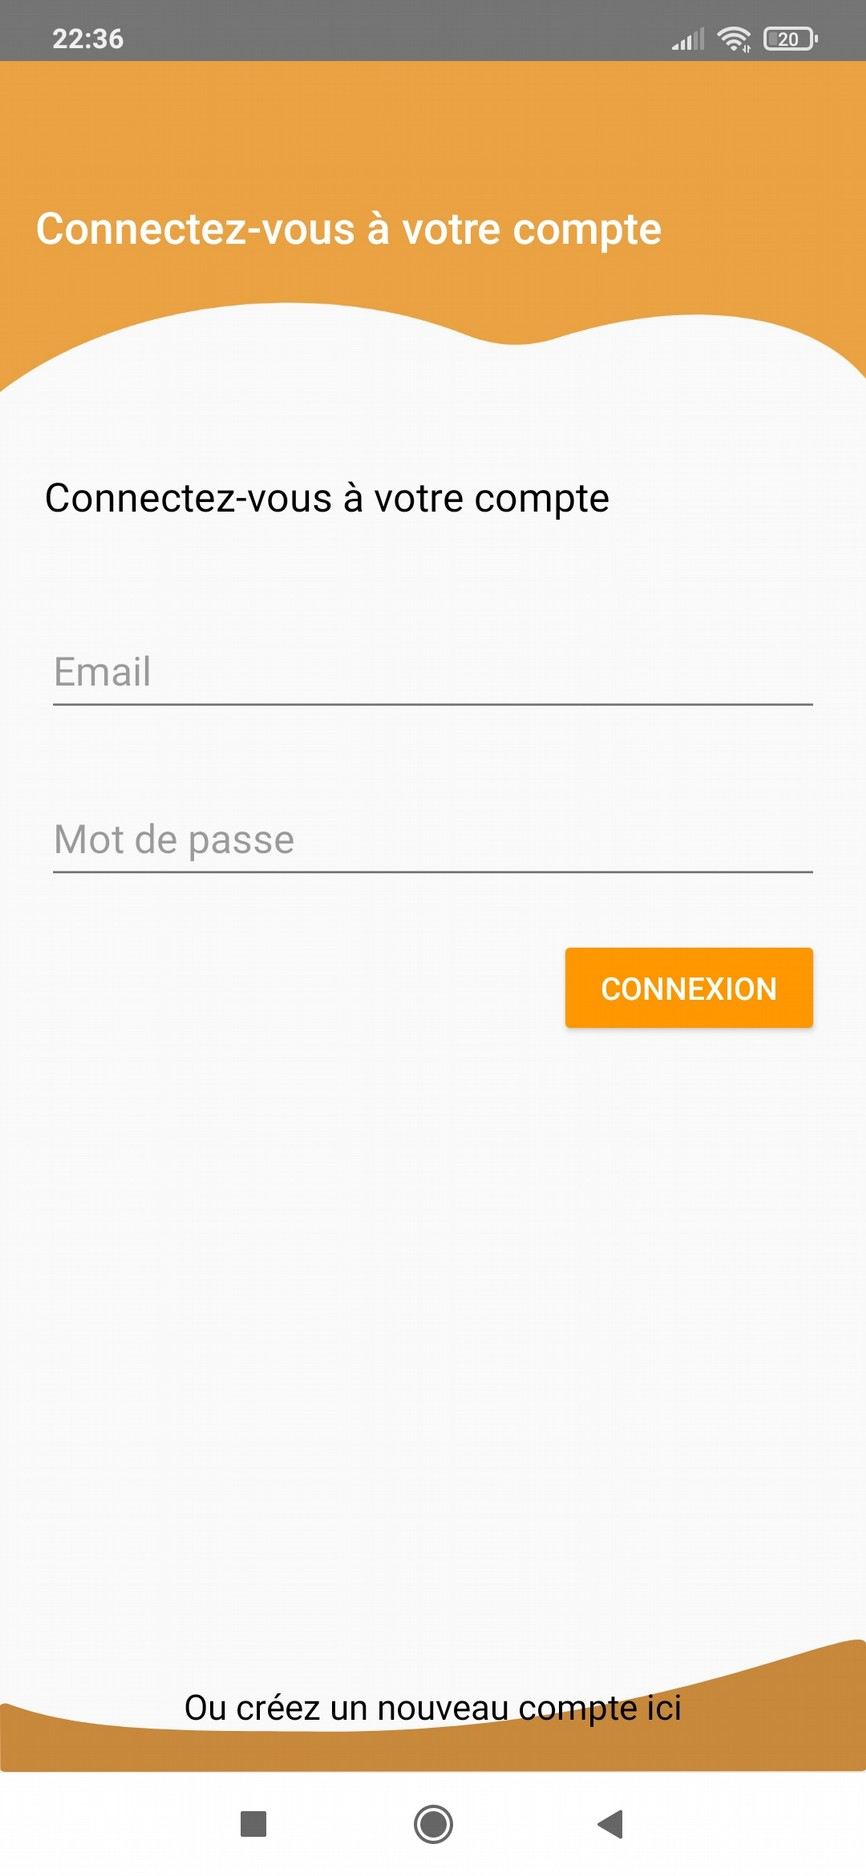
\includegraphics[scale=0.152]{connexion.png}
        %\caption{(Page de connexion)}
    \end{tabular}
    \begin{tabular}{@{}c@{}}
        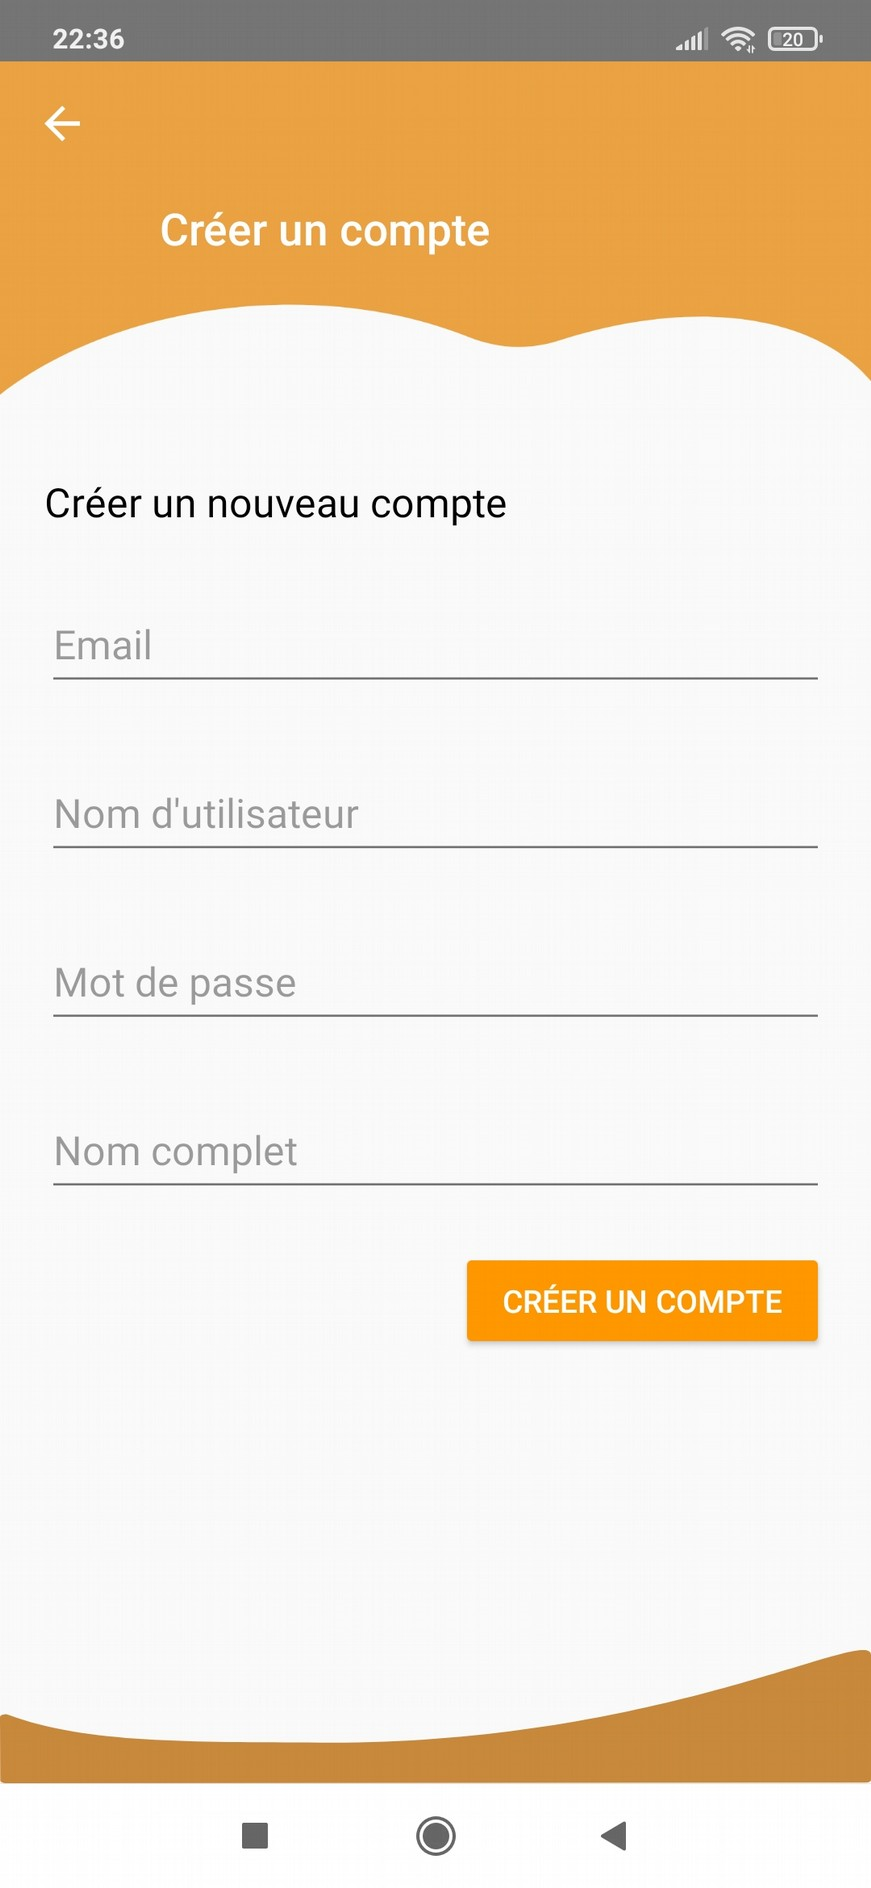
\includegraphics[scale=0.152]{creer_compte.png}
        %\caption{(Clic sur Créer un nouveau compte)}
    \end{tabular}
\end{figure}

Si l’utilisateur possède déjà un compte, il pourra alors se connecter à un compte déjà existant via la rubrique "Connectez-vous à votre compte". Il suffira qu’il entre son adresse email et son mot de passe et il sera rediriger vers l’écran d’acceuil principal de \textbf{Dodo’Cuisto}.\\

\begin{figure}
    \center
    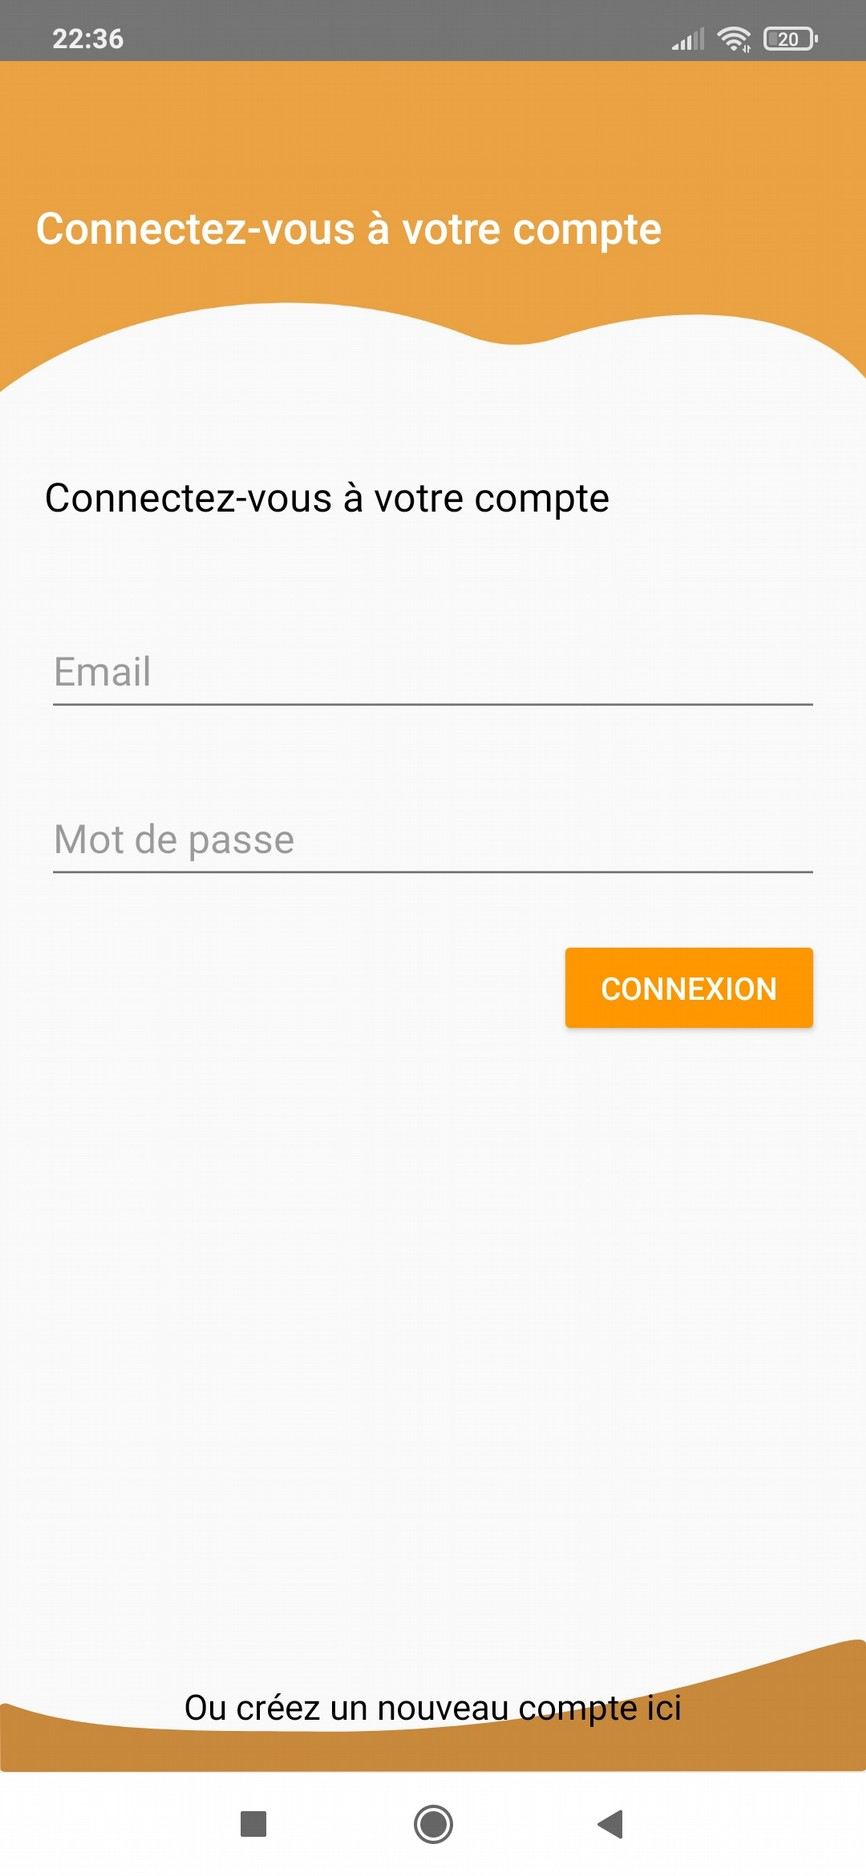
\includegraphics[scale=0.15]{connexion.png}
    \caption{(page de connexion)}
\end{figure}

Sur la page d’acceuil se trouve toute les recettes disponible que ce soit les plats ou les desserts, l’utilisateur pourra faire glisser à droite ou à gauche pour choisir quelle catégorie de recette il souhaite voir. Il peut également écrire directement dans la barre de recherche, le nom de la recette
qu’il souhaiterai consulter.\\

Clic sur une recette par exemple \textit{"Rougail Saucisse"} depuis la page d’acceuil :
Il aura alors le choix de le consulter, le modifier ou le supprimer.
Si l’utilisateur décide de consulter la recette, il aura la possibilité de faire glisser à gauche ou à droite pour voir les ingrédients et les instructions de la recette.

\begin{figure}
    \centering
    \begin{tabular}{@{}c@{}}
        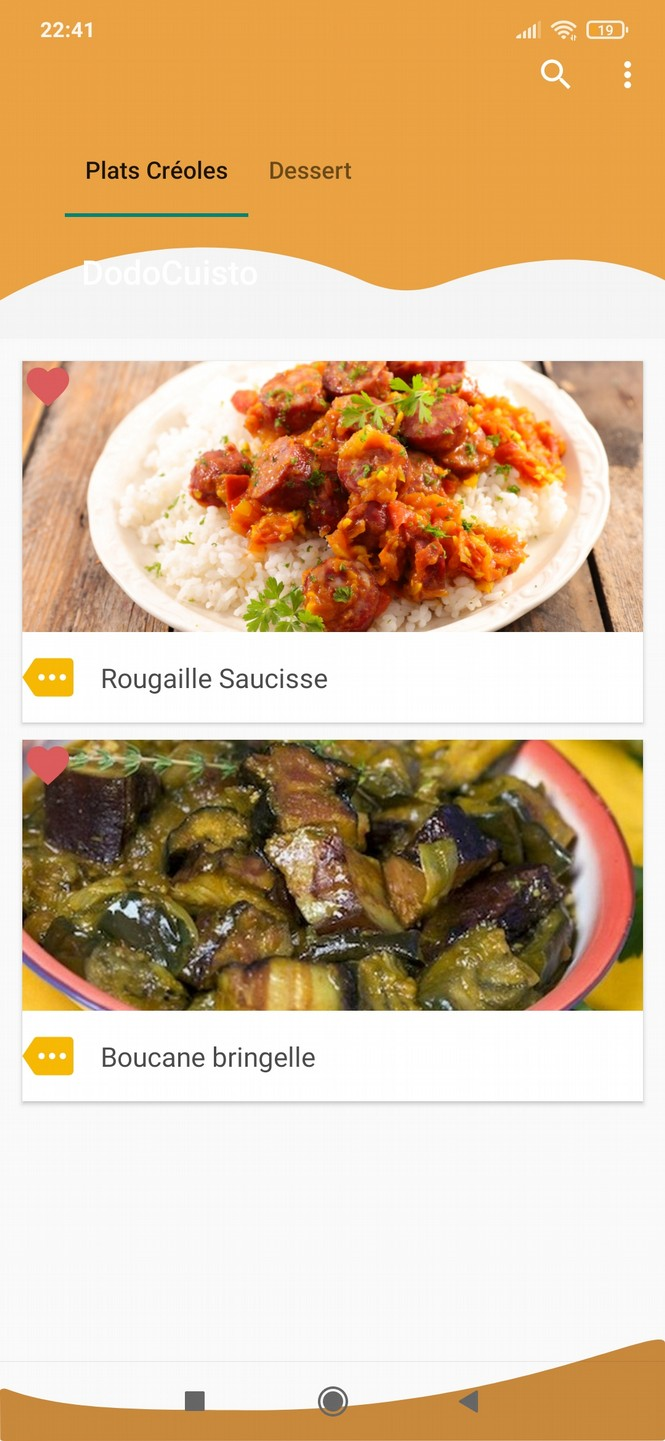
\includegraphics[scale=0.152]{acceuil.png}
        %\caption{(Page de connexion)}
    \end{tabular}
    \begin{tabular}{@{}c@{}}
        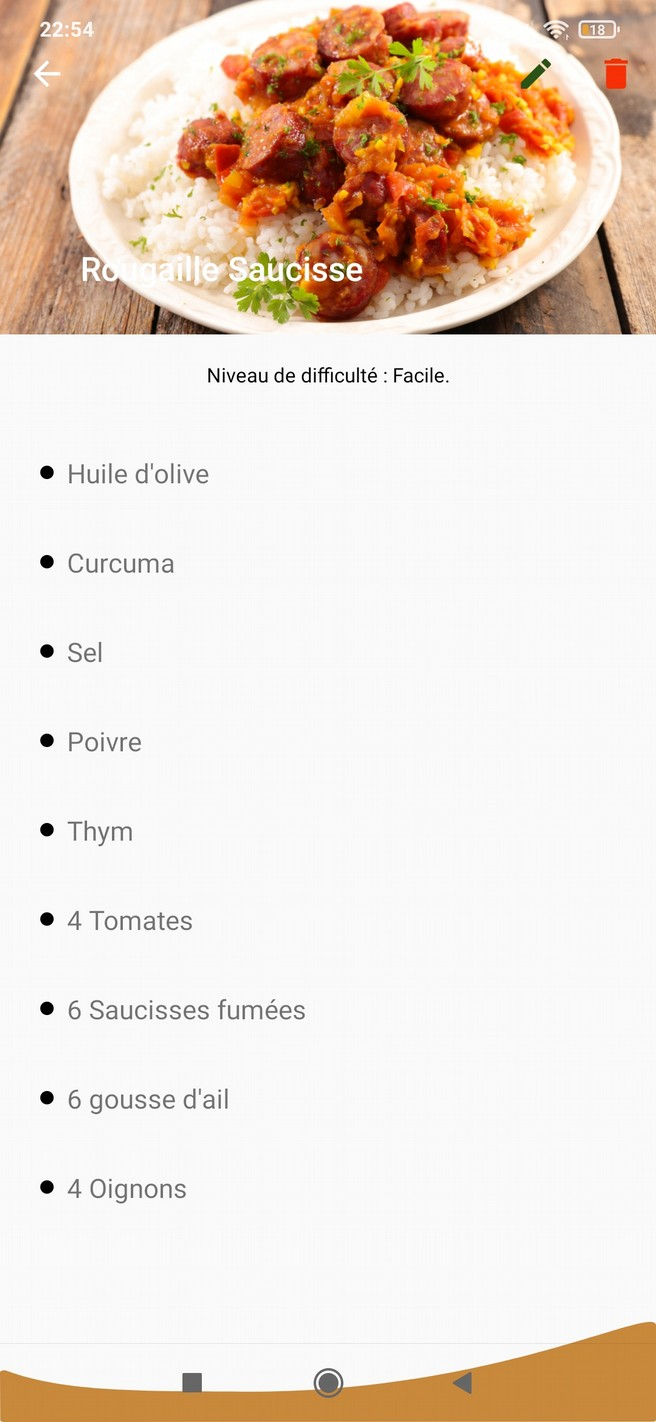
\includegraphics[scale=0.152]{ingrdient.png}
        %\caption{(Clic sur Créer un nouveau compte)}
    \end{tabular}
    \begin{tabular}{@{}c@{}}
        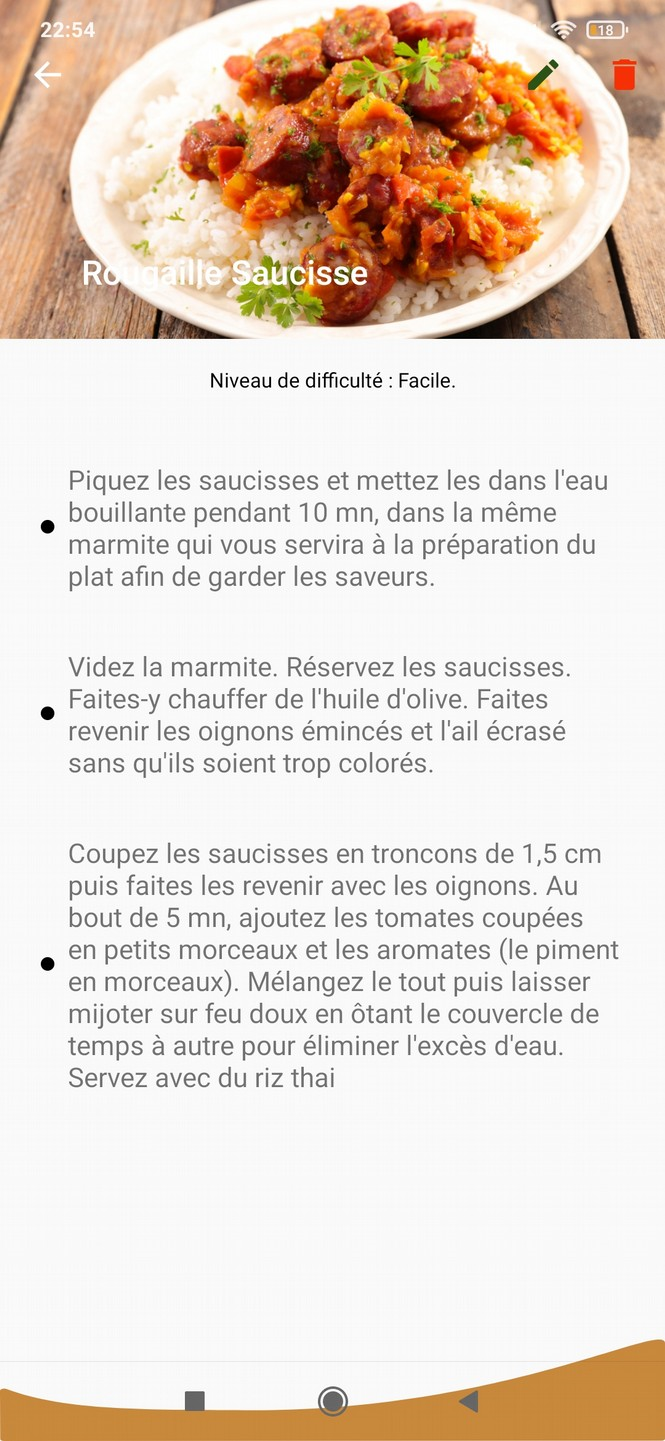
\includegraphics[scale=0.152]{direction.png}
        %\caption{(Clic sur Créer un nouveau compte)}
    \end{tabular}
\end{figure}

Toujours depuis l’écran d’acceuil, en cliquant sur les trois petits points en haut à droite de l’écran, l’utilisateur de \textbf{Dodo’Cuisto} pourra ajouter une nouvelle recette ou se déconnecter.\\

Clic sur \textit{"Nouvelle recette"} depuis l’écran d’acceuil : Des informations seront demandées à l’utilisateur pour pouvoir ajouter une nouvelle recette tel que le nom de la recette, une image illustrative et une courte description de la recette. Lorsque l’utilisateur aura donner tout ces renseignements il pourra cliquer sur "Suivant" et il sera rediriger vers une nouvelle page.

\begin{figure}
    \center
    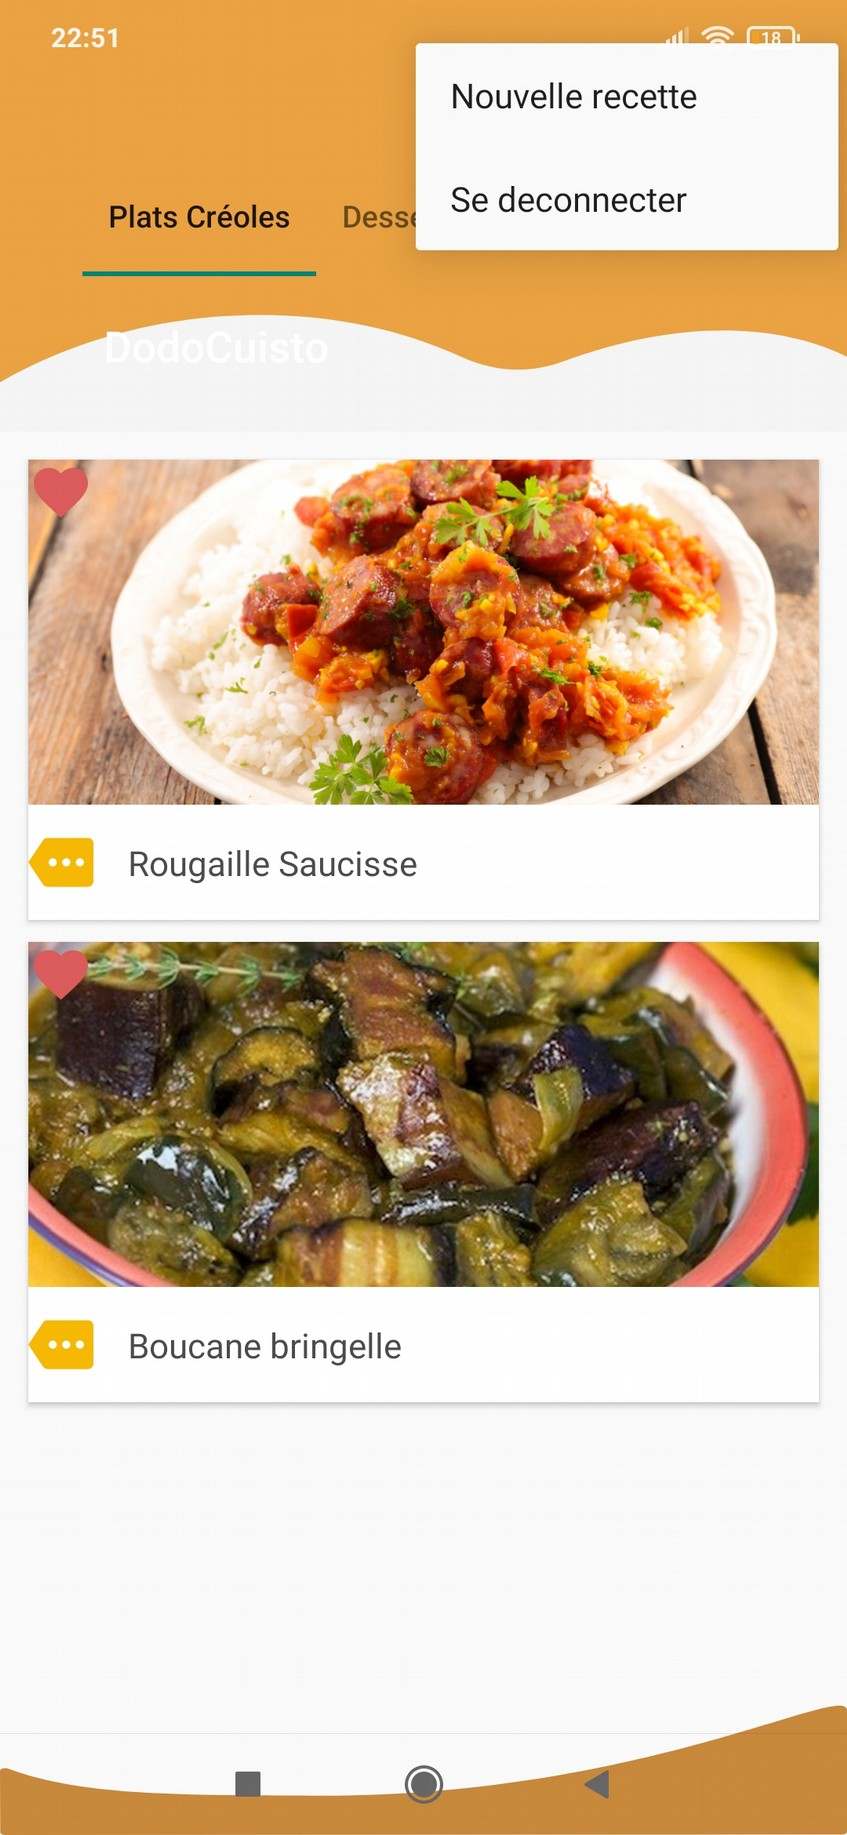
\includegraphics[scale=0.152]{latexImage_eb004d55af912ff8e84e9b6d41a55581.png}
\end{figure}

Sur cette nouvelle page, il devra ajouter les ingrédients de sa recette. L’utilisateur pourra alors ajouter autant d’ingrédients qu’il le souhaite en cliquant sur \textit{"Ajouter"}, et lorsqu’il aurait fini d’ajouter tout les ingrédients nécessaire à sa recette, il cliquera sur "Suivant" et il sera de nouveau rediriger vers une nouvelle page.\\

Dans cette nouvelle page finale, on doit écrire les instructions pour notre recette. Et comme précédemment, on peut alors ajouter autant d’instructions qu’on le souhaite en cliquant sur \textit{"Ajouter"}, et lorsqu’on a fini d’écrire tout les instructions nécessaire à la réalisation de cette recette, on clique sur \textit{"Terminer"} et on sera rediriger sur la page d’acceuil.

\begin{figure}
    \centering
    \begin{tabular}{@{}c@{}}
        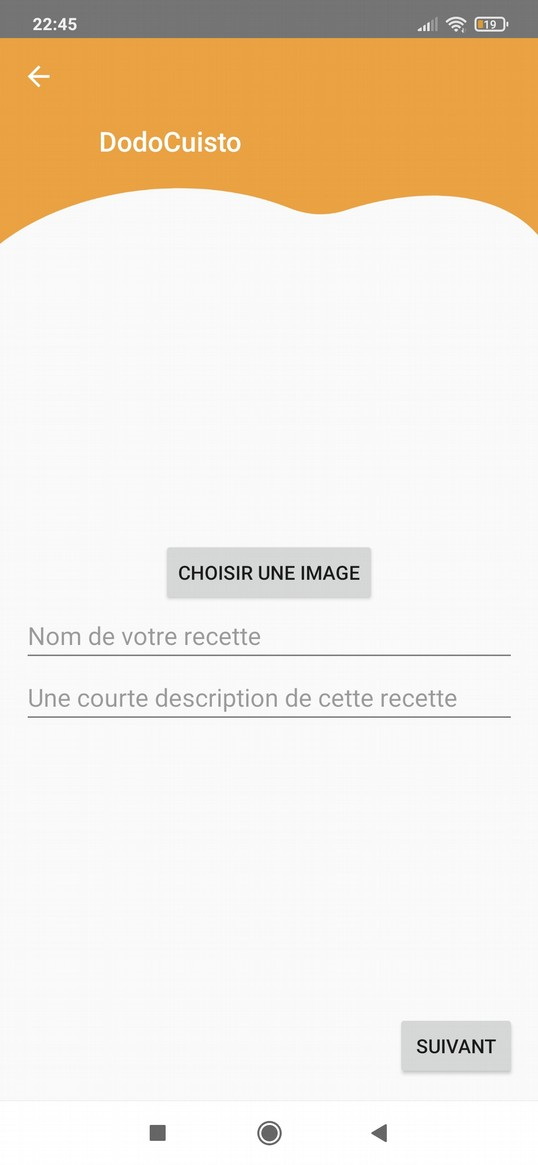
\includegraphics[scale=0.2]{add_image.png}
        %\caption{(Page de connexion)}
    \end{tabular}
    \begin{tabular}{@{}c@{}}
        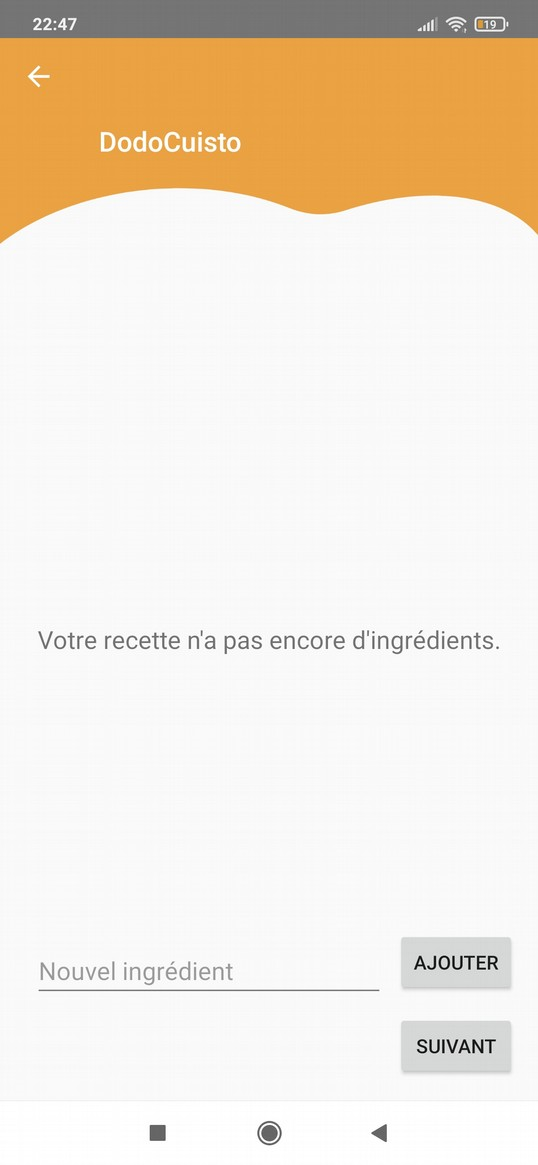
\includegraphics[scale=0.2]{add_ingredients.png}
        %\caption{(Clic sur Créer un nouveau compte)}
    \end{tabular}
    \begin{tabular}{@{}c@{}}
        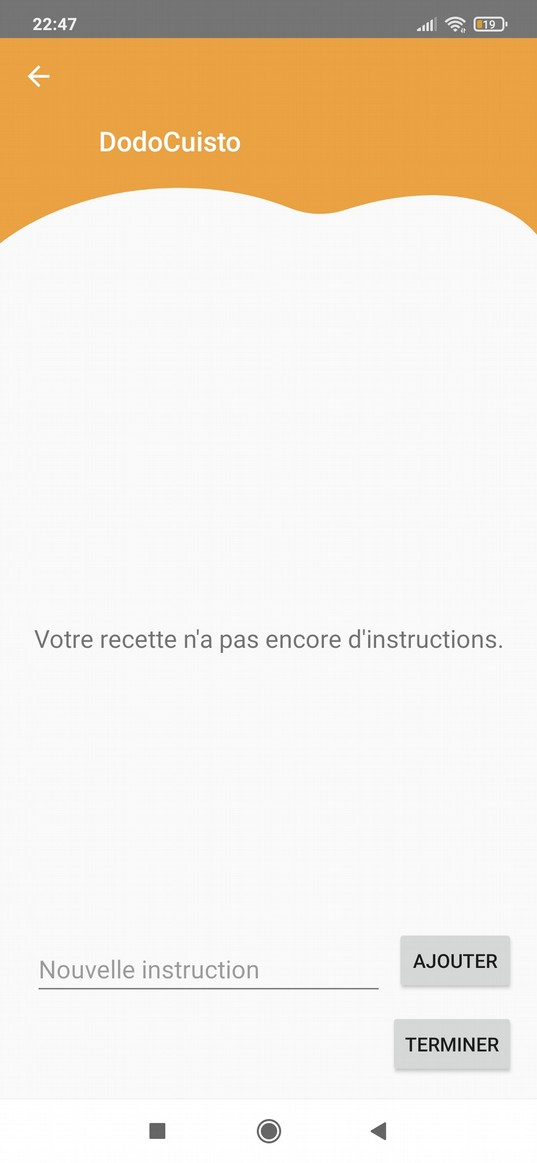
\includegraphics[scale=0.2]{instruction.png}
        %\caption{(Clic sur Créer un nouveau compte)}
    \end{tabular}
\end{figure}

\subsection{\textcolor{red}{Lecture des données avec DB Browser for SQLite}}

Nous avons utilisé le logiciel \textbf{DB Browser for SQLite} pour consulter la base de données locale et de s’assurer le bon fonctionnement de celle-ci. Ce logiciel gratuit et libre permet de créer et manipuler des bases de données sans avoir besoin d’un serveur.\\

Pour consulter notre base de données locale, tout d’abord, nous avons extrait le fichier \textit{"recipesDatabase"}, qui contient toute les données de la base de données locale, à partir d’Android Studio. Pour ce faire, sur Android Studio, on se place dans l’onglet \textit{"Device File Explorer"} et dans le dossier \textit{"database"} on récupère le fichier \textit{"recipesDatabase"} et on lui ajoutera l’extension \textit{".sqlite"}. Il ne reste plus qu’à ouvrir ce fichier avec le logiciel \textbf{DB Browser for SQLite}.\\

\newpage

\begin{center}
    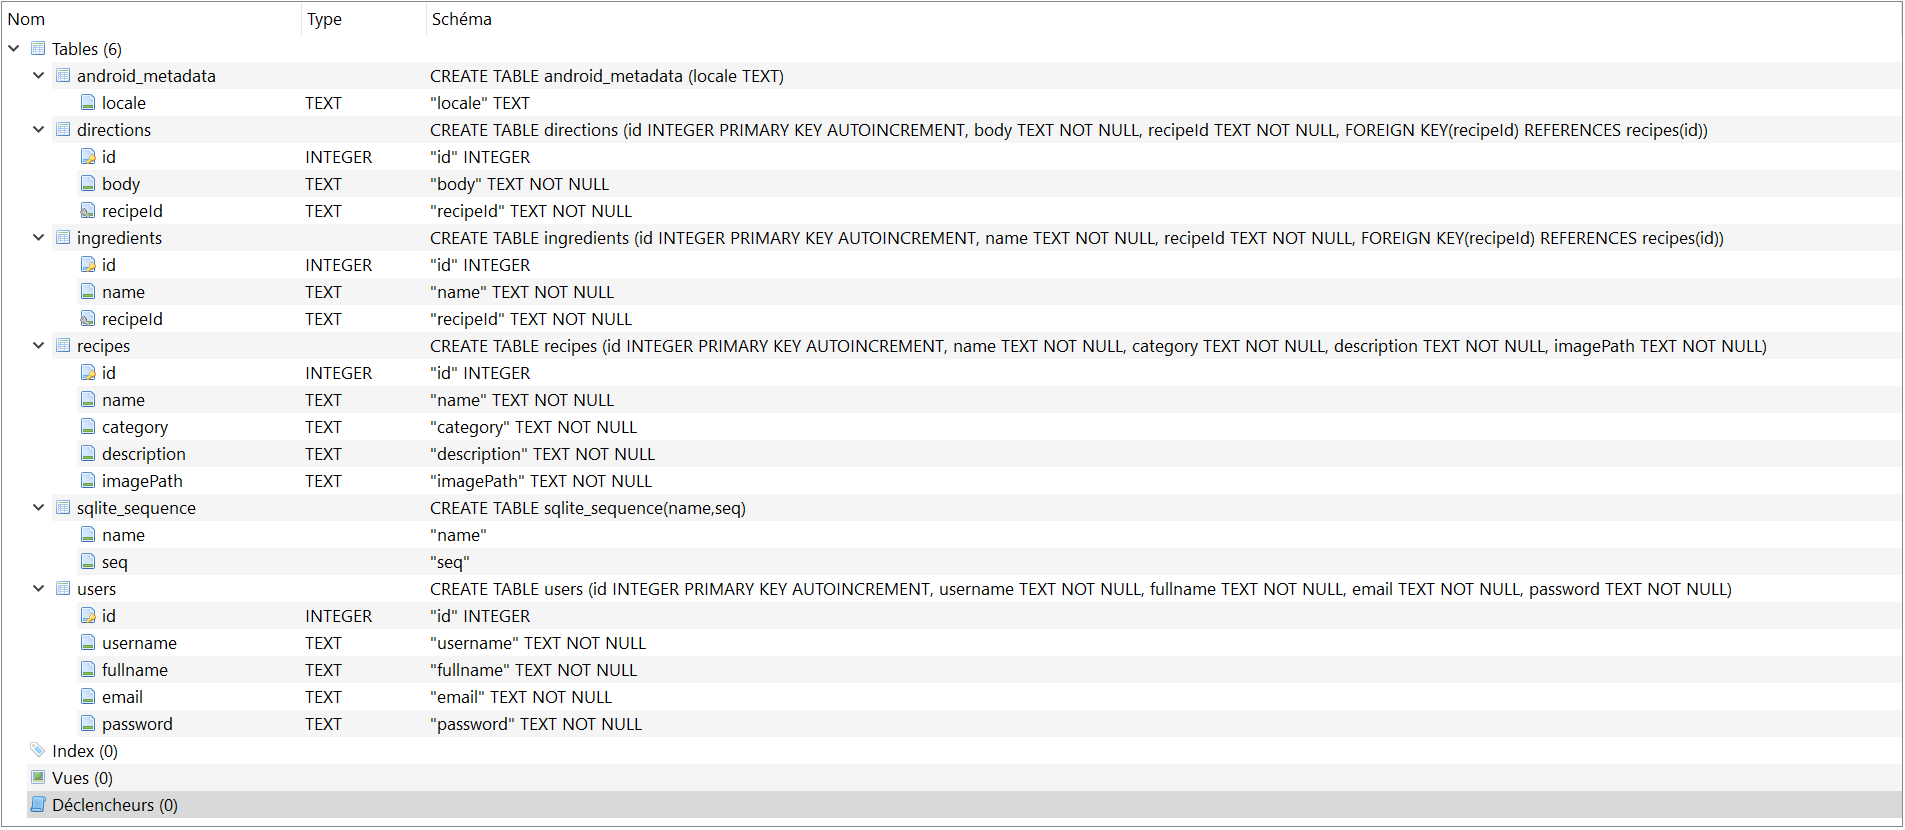
\includegraphics[scale=0.4]{vue_global_bdd.png} 
    %\caption{(Vue global de DB Browser for SQLite)}
\end{center}

Dans l’onglet \textit{"Parcourir les données"} du logiciel, on peux naviguer dans la liste déroulante "table" pour consulter les différentes tables de la base de données.\\

\begin{center}
    \includegraphics[scale=0.4]{ingrédients.png} 
\end{center}

Ici, nous avons la table \textit{"ingredients"}, qui contient tout les ingrédients de toute les recettes disponible dans notre application Dodo’Cuisto. On remarque que tout les ingrédients d’une même recette possède tous le même numéro d’identifiant \textit{"recipeId"}. Nous obtenons la même chose pour la table "directions", qui contient les instructions de recette.\\

\newpage

\begin{center}
    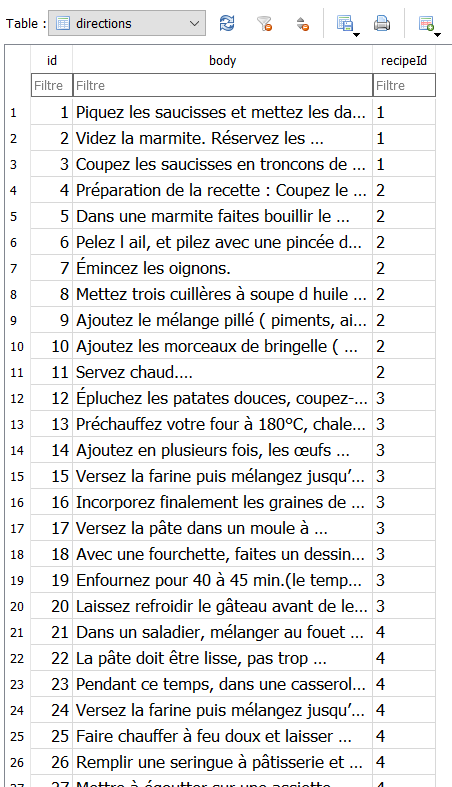
\includegraphics[scale=0.4]{directions.png} 
\end{center}

Nous avons également les tables \textit{"recipes"} et \textit{"users"} qui contiennent respectivement les recettes et les données de l’utilisateur.

\begin{figure}
    \centering
    \begin{tabular}{@{}c@{}}
        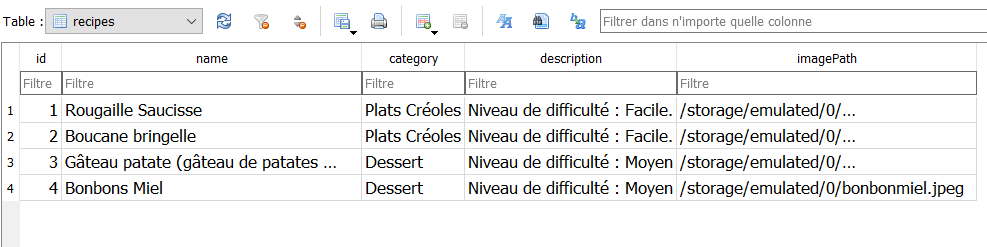
\includegraphics[scale=0.8]{recettes.png}
    \end{tabular}
    \begin{tabular}{@{}c@{}}
        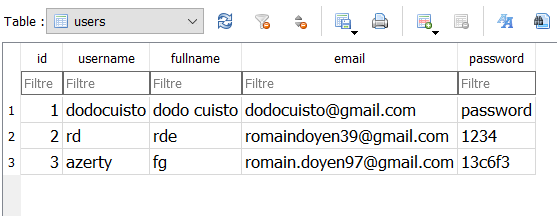
\includegraphics[scale=0.8]{users.png}
    \end{tabular}
    \caption{(Table recipes and Table users)}
\end{figure}

\newpage

%==============================================================================%

\section{\textcolor{red}{Les problèmes rencontrés}}

Nous n’avons pas pu trouver d’image libre de droit pour les recettes créoles dans des banques d’images libres de droits. Nous étions obligés de prendre les images sur Google image.\\

\subsection{\textcolor{red}{Quelques souci d’affichage}}

Nous avons eu quelques difficultés à faire afficher certaines fonctionnalités de l’application. Quand on clique sur une recette, les fragments \textit{"ingrédients"} et \textit{"instructions (direction)"} n’apparaissent pas à l’écran. En effet, cela est une indication visuelle qui permet à l’utilisateur de mieux se repérer lorsqu’il navigue entre les ingrédients et les instructions de recettes, mais il n’empêche en aucun cas le bon usage de l’application.\\

\subsection{\textcolor{red}{Problème avec certaines fonctionnalités}}

Nous avons également eu quelques problème à faire fonctionner correctement certaines fonctionnalités de \textbf{Dodo’Cuisto}. La barre de recherche située dans la page d’acceuil de l’application ne fonctionne pas correctement. En effet, la barre de recherche a beaucoup de difficulté à rechercher les recettes disponible dans la liste des recettes.\\

L’option \textit{"favoris"} qui permet notamment de mettre en favoris les recettes préférés de l’utilisateur afin de mieux le répertorier dans la liste des recettes, rencontre également un souci de fonctionnement.\\

\begin{center}
    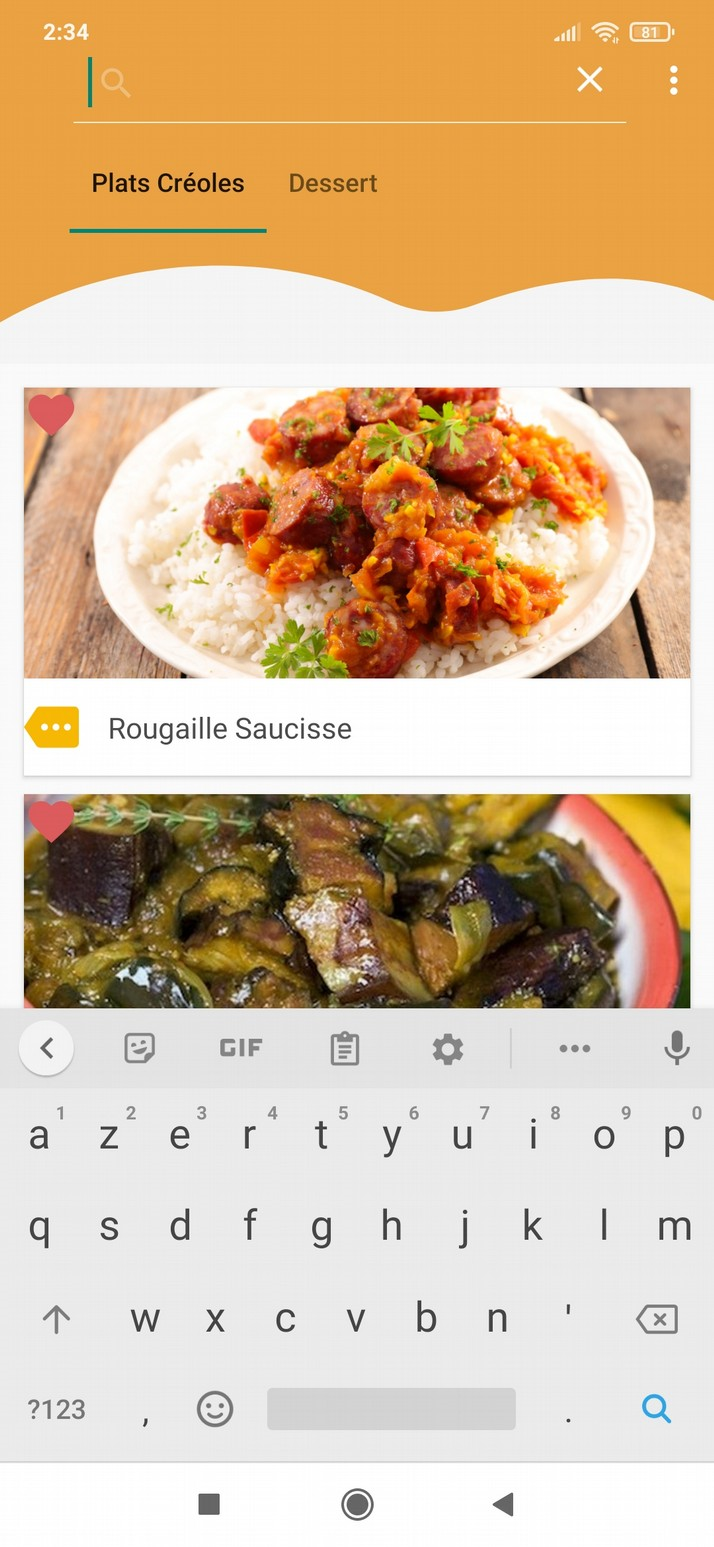
\includegraphics[scale=0.2]{recherche.png} 
\end{center}

Lorsqu’on souhaite cliquer sur le \textit{"coeur rouge"} situant en haut à gauche des recettes, symbolisant l’option "favoris", le \textit{"coeur rouge"} reste figer et ne fonctionne pas.\\

%==============================================================================%

\section{\textcolor{red}{L'un des principaux challenges rencontrés}}

L'un des principaux challenge est l'affichage des recettes. Pour cela nous avons eu besoin d'implémenter une \textbf{TabLayout} pour les ingrédients et à la fois pour les instructions (direction)  \textbf{ViewRecetteActivity}

\begin{center}
    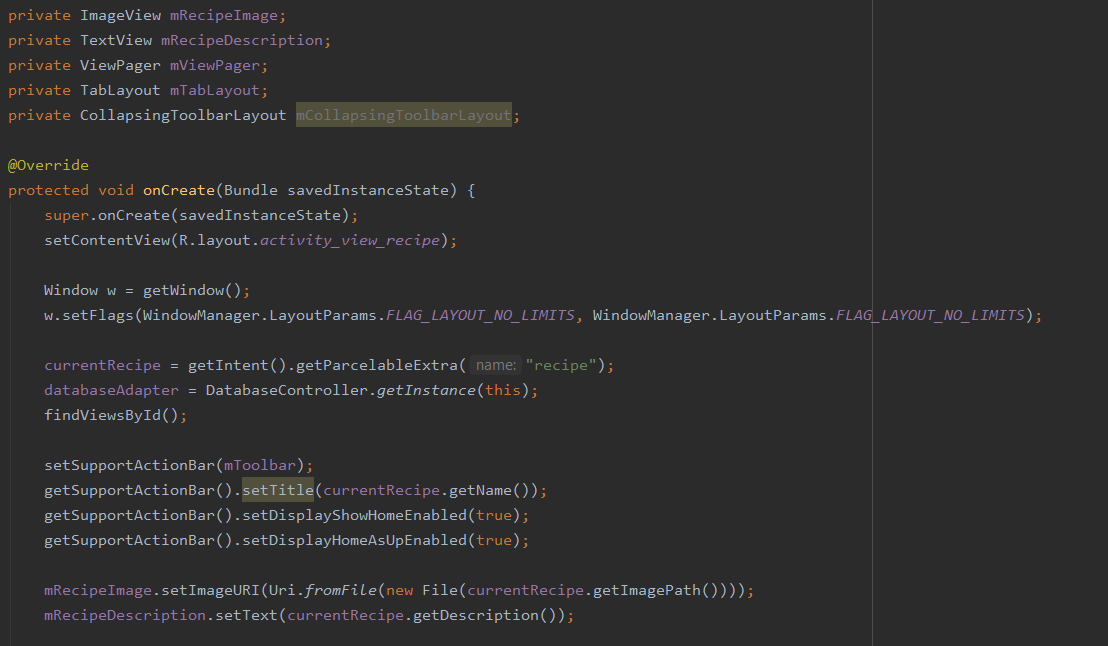
\includegraphics[scale=0.7]{viewrecetteacti.png} 
\end{center}

Ensuite il a fallut adapter l'affichage en fonction du \textbf{TabLayout} dans lequel on se trouve par l'intermédiaire \textbf{CollapsingToolbarLayout} dans le \textbf{MainActivity}, au début nous avons utilisé des conditions puis on s'est vite rendu compte que le \textbf{switch case} était beaucoup approprié. 

\newpage

\begin{center}
    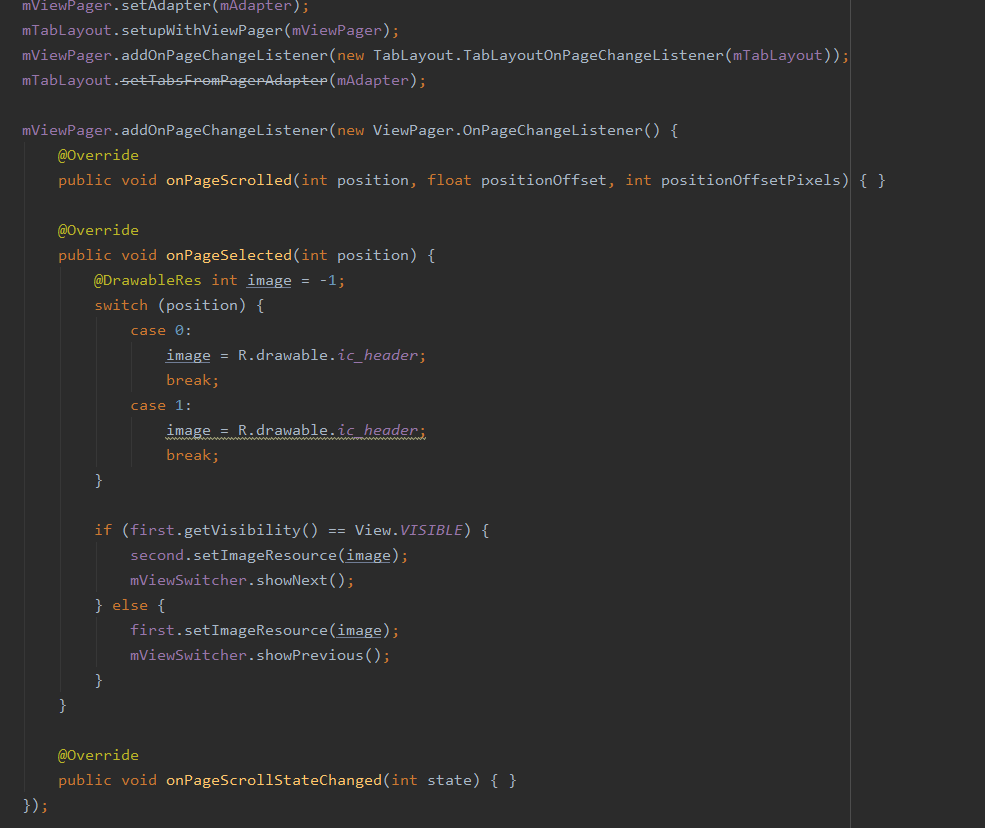
\includegraphics[scale=0.7]{mainacti.png} 
\end{center}

%==============================================================================%

\section{\textcolor{red}{L'inconvénient d'un code en MVC}}

Lors du développement de l'application nous avons utilisé la technologie \textbf{MVC} \textit{comme dit plus haut} afin de séparer les tâches, la logique de l'interface mais cela implique une augmentation de la complexité de l’architecture. En effet nous avons rencontré été confronté a un problème de coordination niveau de l'interfacage des couches.\\

Aussi par l'énorme quantité de fichier à manipuler, en effet la séparation des différentes couches nécessite la création de plus de fichiers (3 fois pour les différentes couches).\\

Mais cela à permis la reutilisabilite de certaine couche 

%\newpage
%==============================================================================%

\section{\textcolor{red}{Quelques points délicats/intéressants}}

\subsection{\textcolor{red}{Le stockage des données avec SQLite}}

Nous avons utilisé la base de données \textbf{SQLite} pour notre application. \textbf{SQLite} est intégrée dans chaque appareil \textbf{Android}. Son utilisation sous \textbf{Android} ne nécessite pas de configuration ou d'administration de la base de données.\\

Pour créer et mettre à jour une base de données dans notre application \textbf{Android}, nous avons créé une classe de nom \textbf{SQLiteDatabaseHelper} qui hérite de \textbf{SQLiteOpenHelper}. Dans le constructeur de notre classe, nous avons appelé la méthode \textbf{super()} de \textbf{SQLiteOpenHelper}, en précisant le nom de la base de données et sa version actuelle.\\

\begin{figure}
    \center
    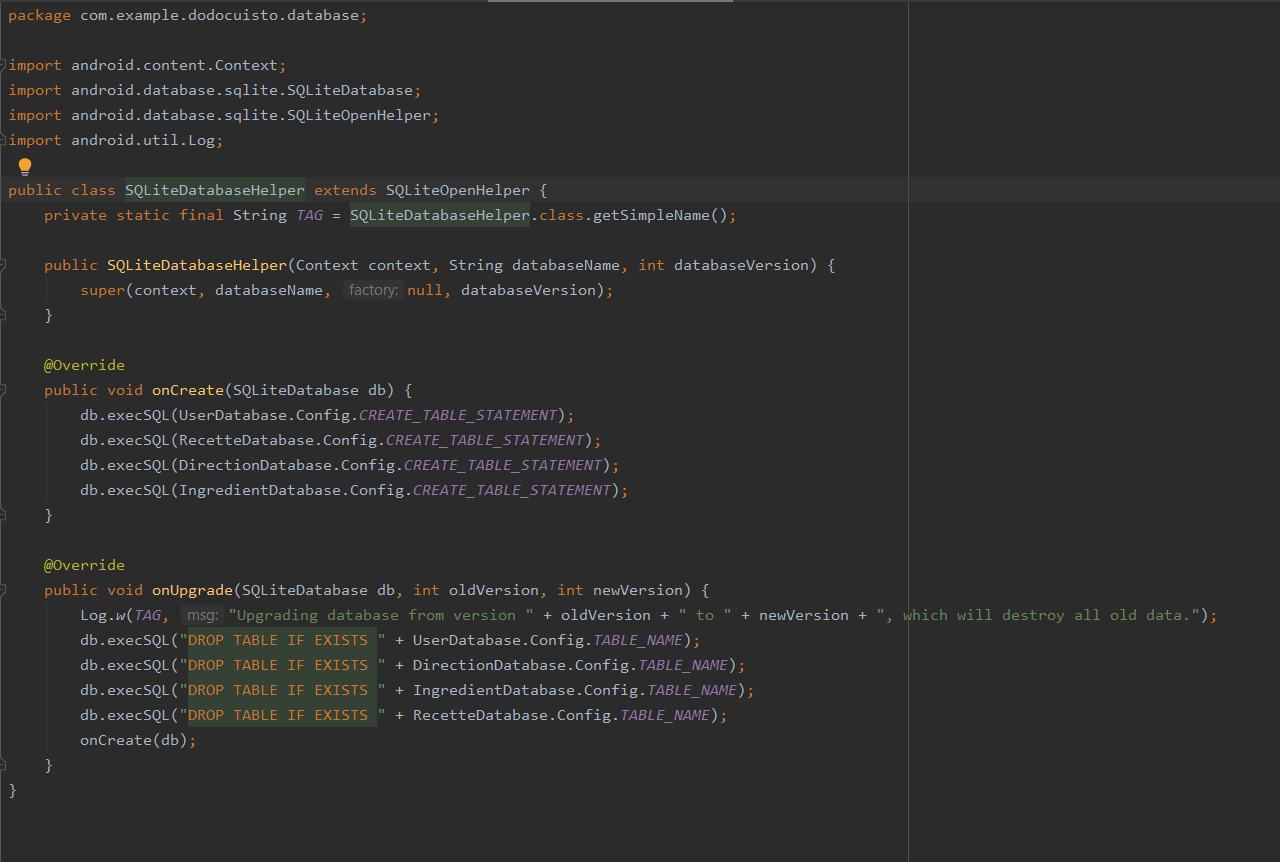
\includegraphics[scale=0.5]{sqlhelper.png}
\end{figure}

Dans la classe \textbf{SQLiteDatabaseHelper}, nous avons redéfini les méthodes suivantes pour créer et mettre à jour notre base de données :
\begin{itemize}
    \item \item \textbf{onCreate():} Appelé lorsque la base de données est créée pour la première fois.
    \item \item \textbf{onUpgrade():} Appelé lorsque la base de données doit être mise à jour.\\
\end{itemize}

La méthode \textbf{onCreate()} sera appelée par le framework pour accéder à une base de données qui n'est pas encore créée. Tandis que la méthode \textbf{onUpgrade()} sera appelée si la version de la base de données est augmentée dans le code de notre application. Cette méthode nous permet de mettre à jour un schéma de base de données existant ou de supprimer la base de données existante et la recréer par la méthode \textbf{onCreate()}.\\

Ces deux méthodes reçoivent en paramètre un objet \textbf{SQLiteDatabase} qui est la représentation Java de la base de données.
\textbf{SQLiteDatabase} est la classe de base pour travailler avec une base de données \textbf{SQLite} sous \textbf{Android} et fournit des méthodes pour ouvrir, effectuer des requêtes, mettre à jour et fermer la base de données.\\

Plus précisément, \textbf{SQLiteDatabase} fournit les méthodes \textbf{insert()}, \textbf{update()} et \textbf{delete()}. En outre, elle fournit la méthode \textbf{execSQL()}, qui permet d'exécuter une instruction \textbf{SQL} directement.\\

\begin{figure}
    \center
    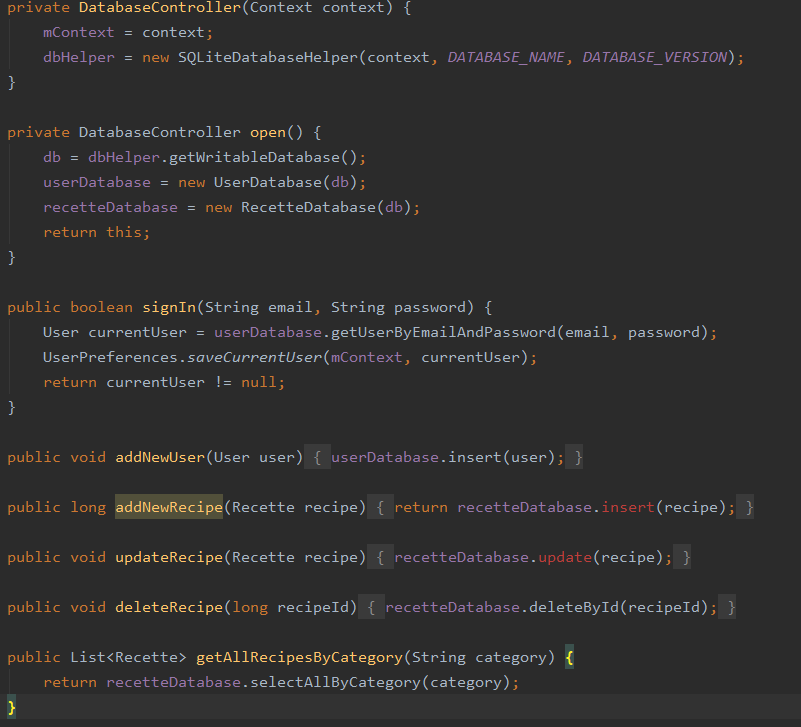
\includegraphics[scale=0.7]{insert_update_delete.png}
\end{figure}

L'utilisation de ces méthodes sont directement implémenté dans la class \textbf{DatabaseController}.

\newpage

%==============================================================================%

\section{\textcolor{red}{Conclusion}}

Pour conclure, avec son choix de sujets libre, ce projet nous a permis de faire preuve de créativité et d’imagination. En effet, grâce à \textbf{Android studio} et \textbf{Xcode} nous avons appris et découvrir les différentes étapes d’un processus de développement d’une application et surtout de pouvoir les réaliser soi-même. Nous sommes assez satisfait de notre travail, notre application est plutôt bien
réussi.

\subsection{\textcolor{red}{Les points à améliorer}}

Nous avons réussi à développer notre application avec les fonctionnalitées de base que nous attendions. Cependant, nous pouvons citer quelques points à améliorer comme par exemple :

\begin{itemize}
    \item L’ergonomie de l’application : rendre \textbf{Dodo’Cuisto} encore plus efficace à utiliser
    \item Ajout d’un espace commentaire sur les recettes : donner son avis sur les recettes
    \item Possibilité de personnaliser son profil(mettre une photo de profil, ajouter un numéro de téléphone etc...)
    \item Une barre de recherche et option de favoris plus efficace et ergonomique
\end{itemize}

%==============================================================================%

\section{\textcolor{red}{Bibliographie}}

%%% La bibliographie:
\cite{androidDoc} 
\cite{SQLite}
\cite{androidDoc}
\cite{Image}
\cite{OpenClassRoomYoutube}
\cite{TutoAndroid}

Nous nous sommes inspirés de plusieurs exemples de code sur des sites de tutoriel ou sur Youtube, de solutions trouvées sur StackOverflow, etc. . . qui dans la plupart des cas ont dû être re adaptées afin de convenir à notre contexte.\\

Citées ci-dessous, quelques aides qui nous ont beaucoup aidé :

\bibliographystyle{plain}
\bibliography{ma_biblio}

\end{document}
